\documentclass[A4,10pt]{article}

%% DO NOT MODIFY THIS PREAMBLE
\usepackage{hyperref}
\usepackage{graphicx}
\usepackage{enumitem}
\setlist[itemize]{noitemsep}
\setlist[enumerate]{noitemsep}
\setlength{\parindent}{0cm}
\setlength{\parskip}{1ex}
\setlength{\columnsep}{25pt}

\textwidth=14cm
\textheight=23cm
\setlength{\unitlength}{0.5cm}
\setlength{\parindent}{0.0cm}
\setlength{\parskip}{0.5ex}
\raggedbottom
\sloppy
%\addtolength{\evensidemargin}{-5cm}
\addtolength{\oddsidemargin}{-3cm}
\addtolength{\topmargin}{-2cm}

\renewcommand{\baselinestretch}{1.2} 

%% ADD YOUR PACKAGES HERE
\usepackage{minted} % Add this line to include the minted package

\sloppy

% Your name
\author{Lukas Radovansky \\ Technische Universit\"at M\"unchen}

\title{Master Lab IoT}

% Date of your talk
\date{20.1.2025}


\begin{document}

\maketitle
\newpage
\tableofcontents
\newpage

\section{Background for grading (0.5 page)}
\begin{itemize}
	\item \textbf{General overview of your schedule including longer leave of absence (e.g., vacations) to explain missing data:}
	\begin{itemize}
		\item I was on Christmas leave from 21.12.2024 to 2.1.2025.
	\end{itemize}

	\item \textbf{Hardware problems:}
	\begin{itemize}
		\item At the beginning of the semester, I encountered a problem with my ESPs that couldn't maintain a stable connection to the FRITZBOX router.
		\item I spent a lot of time trying to fix the issue, but I couldn't find a solution.
		\item In the end, I asked my landlord to give me the router credentials to debug the issue, which he refused.
		\item Instead, he provided me with a small router that I connected to the FRITZBOX. This solved the issue, and I was able to continue with the project.
		\item However, the router was not able to maintain a stable connection all the time and sometimes had to be restarted.
	\end{itemize}

	\item \textbf{Credentials changed for the Digital Twin:}
	\begin{itemize}
		\item There were no credentials changed for the Digital Twin app.
	\end{itemize}
\end{itemize}

\section{Your setup at home (1 page)}

\begin{itemize}
	\item \textbf{Scale map and sensor placement:}
	\begin{itemize}
		\item Present the scale map with the placement of the sensor and the observed area.
	\end{itemize}
\end{itemize}

\begin{figure}[H]
\centering
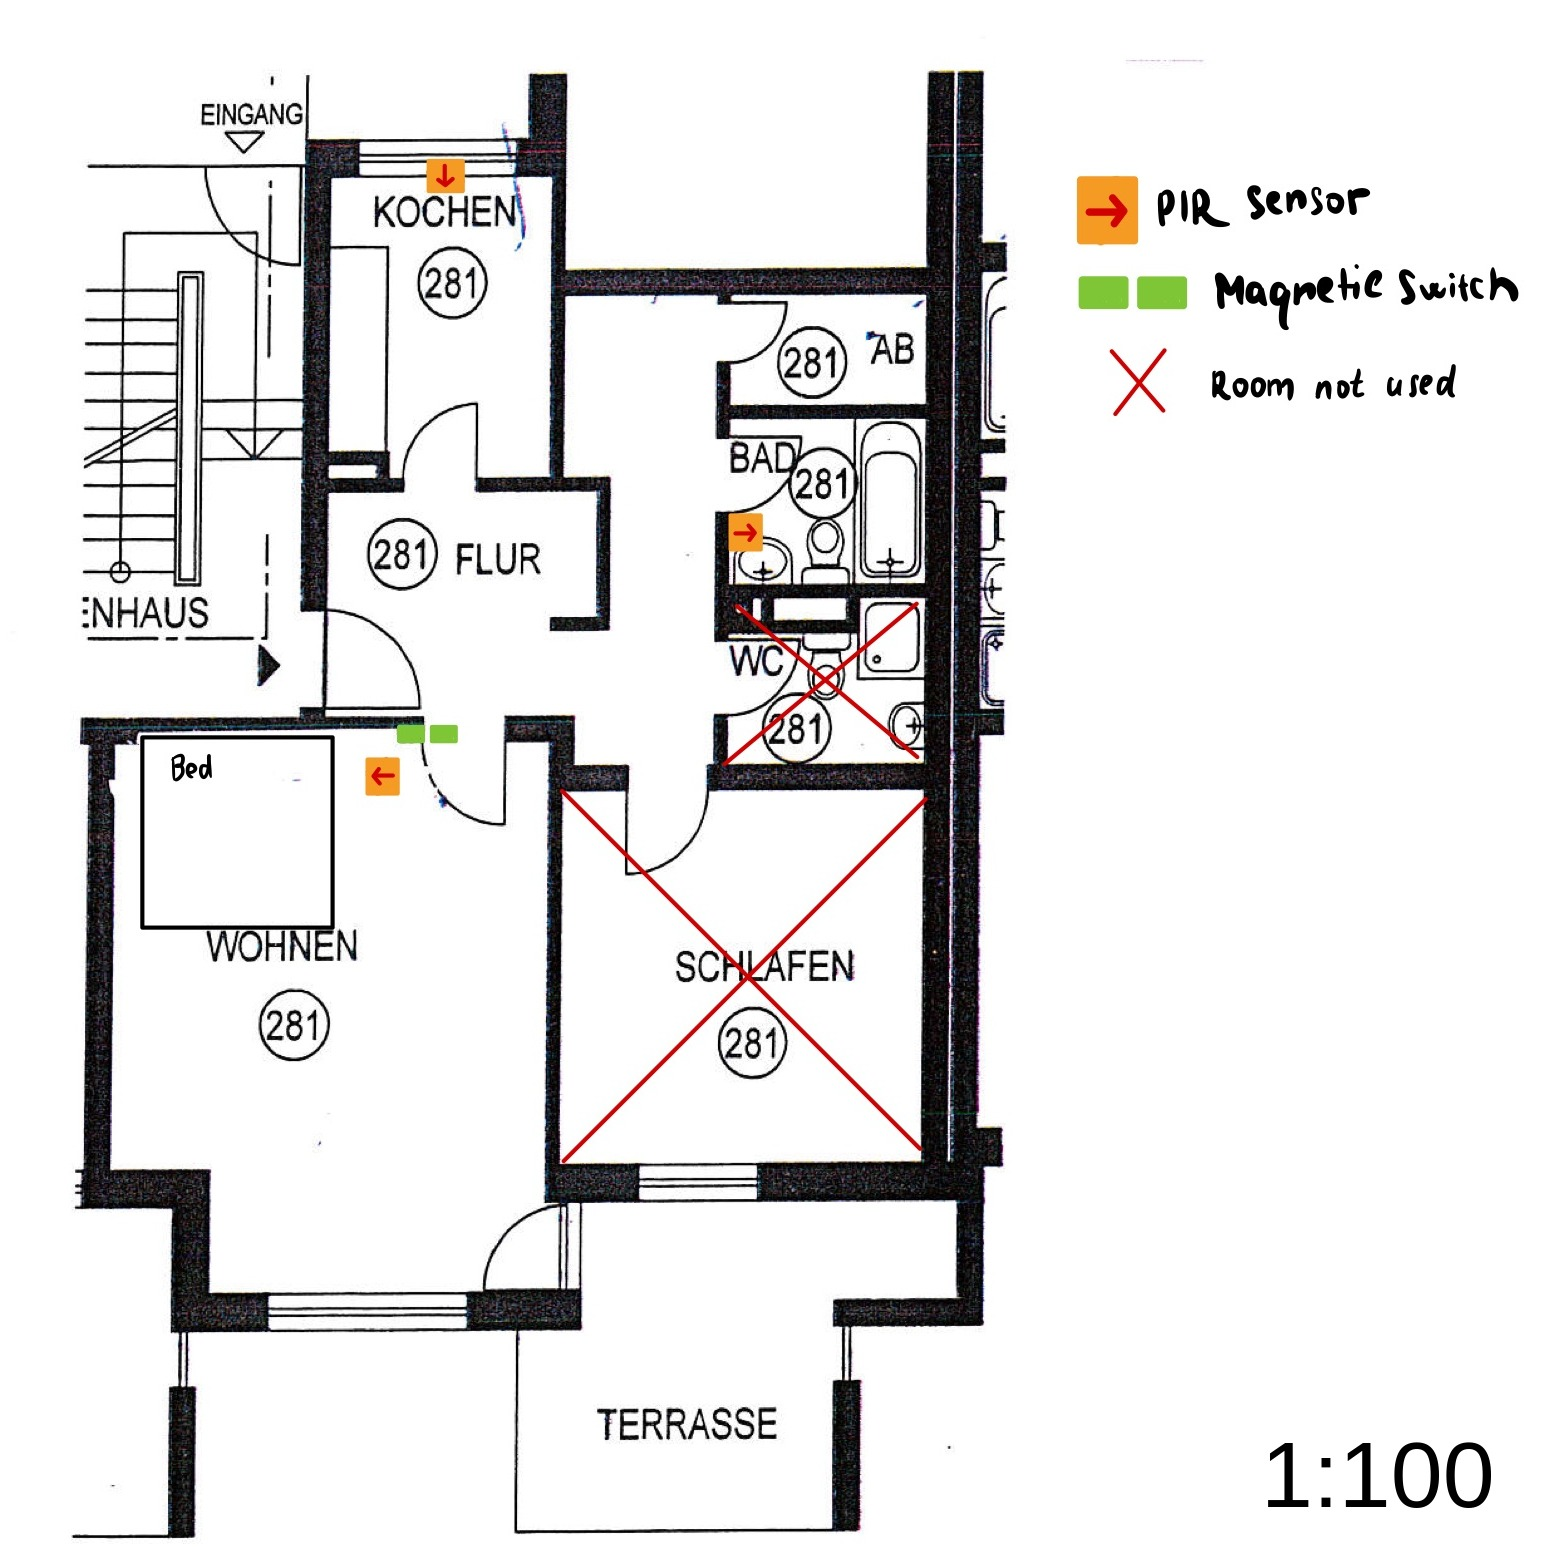
\includegraphics[width=0.6\textwidth]{grundriss.jpeg}
\caption{Scale map illustrating the sensor placement and the monitored area. The scale is 1:100. Red arrows indicate the orientation of the PIR sensors. Crossed-out areas are not part of the rented section of the flat.}
\label{fig:scale_map}
\end{figure}

\begin{itemize}
	\item \textbf{Challenges from positioning:}
	\begin{itemize}
		\item The Sensor in the kitchen triggered false positives if the door to the kitchen were opened and someone was in the hallway. 
		\item The sensor placed in bathroom could be affected by the steam from the shower, however the device seems to survive the humidity well.
		\item I have deployed exactly one ESP with a Magnetic Switch and PIR sensor simultaneously in my apartment. It has been placed in the bedroom. The PIR sensor was pointing towards the bed area, and the magnetic switch was placed on the entrance door. The idea was to track the sleep time of the patient. If the doors remained open, the sensor was still active, and no bed area events were recorded. This was done on purpose because I know that every time the patient goes to sleep, he will close the door first.
	\end{itemize}
	\item \textbf{Setup information:}
	\begin{itemize}
		\item Sharing the flat with another person and a cat presented additional challenges in completing some tasks for this seminar.
		\item Occasionally, a third person (the landlord) would be present in the flat once or twice a week to work from the crossed-out room on the apartment map. The landlord also used the kitchen, where one of the PIR sensors was placed.
		\item Throughout the semester, we hosted guests on several occasions (4-5 times), which impacted the data collection process. The highest number of guests was five, during the weekend of December 12-15, 2024.
	\end{itemize}
\end{itemize}

\section{Sensor Development (10 pages)}

\subsection{Challenges (0.5p)}

\begin{itemize}
	\item \textbf{Describe any aspect to consider while grading that impacted the development of your code, such as: programming skills, difficulties in understanding concepts, etc.}
	\begin{itemize}
		\item I had limited experience with embedded systems programming, which required additional time to learn and understand the given tasks.
		\item I was also new to Docker and Kubernetes.
	\end{itemize}
\end{itemize}

\subsection{Sensor Integration (0.5p)}

\begin{itemize}
	\item \textbf{Integration of PIR and Magnetic Sensors}
	
	The integration of PIR sensors with a magnetic switch sensor was achieved through the following steps:

	\begin{enumerate}
		\item \textbf{Hardware Configuration:} 
		\begin{itemize}
			\item \textbf{PIR Sensor} connected to GPIO pin 27.
			\item \textbf{Magnetic Switch Sensor} connected to GPIO pin 33.
		\end{itemize}
		
		\item \textbf{GPIO Initialization:} 
		Both sensors are configured as RTC GPIOs with pull-down resistors to ensure stable low states when inactive.
		
		\begin{minted}[fontsize=\small]{c}
void configure_rtc_gpio() {
    // Initialize PIR sensor GPIO
    rtc_gpio_init(27);
    rtc_gpio_set_direction(27, RTC_GPIO_MODE_INPUT_ONLY);
    rtc_gpio_pulldown_en(27);
    
    // Initialize Magnetic Switch GPIO
    rtc_gpio_init(33);
    rtc_gpio_set_direction(33, RTC_GPIO_MODE_INPUT_ONLY);
    rtc_gpio_pulldown_en(33);
}
		\end{minted}
		
		\item \textbf{Wake-Up Configuration:} 
		Both sensors are set as wake-up sources using the EXT1 mechanism, allowing the ESP32 to wake from deep sleep when either sensor is triggered.
		\begin{minted}[fontsize=\small]{c}
uint64_t wakeup_pins = (1ULL << 27) | (1ULL << 33);
esp_sleep_enable_ext1_wakeup(wakeup_pins, ESP_EXT1_WAKEUP_ANY_HIGH);
		\end{minted}
		
		\item \textbf{Event Handling:} 
		Upon wake-up, the system identifies which sensor triggered the event and processes it accordingly.
		\begin{minted}[fontsize=\small]{c}
void handle_wakeup_reason(){
    if (wakeup_reason == ESP_SLEEP_WAKEUP_EXT1) {
        uint64_t status = esp_sleep_get_ext1_wakeup_status();
        if (status & (1ULL << 27)) {
            // Handle PIR sensor event
        }
        if (status & (1ULL << 33)) {
            // Handle Magnetic switch event
        }
    }
}
		\end{minted}
			\end{enumerate}
\end{itemize}

\subsection{Single Code for All Sensors (1p)}

\begin{itemize}
    \item \textbf{Generic Code Base for Multiple Sensors}
    
    \begin{itemize}
		\item \textbf{Describe how you achieved a generic code base for all your sensors devices. You can include code snippets.}
		\begin{itemize}
			\item Generic code for all devices was achieved by identifying the device based on its MAC address and configuring it accordingly.
			\item Each device needs to be specied in the `main.h` file with its device name, MAC address, ID, MQTT topic, security key, battery information availability, and room ID.
		\end{itemize}
	\end{itemize}

	\begin{minted}[fontsize=\small]{c}
//Struct definition for device information
/**
 * @brief Represents the configuration and metadata for a device.
 *
 * This struct is used to define the properties of an ESP device, including its
 * name, MAC address, ID, MQTT topic, security key, and whether battery information
 * is available. The struct can be used to identify devices and manage their specific
 * configurations within the system.
 */
 typedef struct {
    char* device_name;             // < Name of the device (e.g., "Living Room").
    uint8_t mac_address[6];        // < MAC address of the device (6 bytes).
    int device_id;                 // < Unique identifier for the device.
    char* device_topic;            // < MQTT topic for publishing device data.
    char* device_key;              // < Security key for authenticating with the MQTT broker.
    bool battery_info_available;   // < Indicates if the device provides battery information.
    char* room_id;                 // < Id of the room as named in the InFlux database.
} device_info_t;


// Example of definition of the device in main.h
// (name, mac adress, topic, key, battery info available, room_id)
#define ESP_DEVICE_1 {"Living Room", {0xEC, 0x62, 0x60, 0xBC, 0xE8, 0x50}, 4, 
"1/4/data", "key", true, "livingroombedarea"}

// Read the MAC address and identify the device in the main function:
uint8_t mac_address[6];
esp_read_mac(mac_address, ESP_MAC_WIFI_STA);
identify_device(mac_address);

// The implementation fo the identify_device function
identify_device(mac_address);
/**
 * @brief Identifies the current device based on its MAC address.
 *
 * Matches the MAC address of the device with the pre-configured device list in `main.h`.
 * Sets the device's ID, MQTT topic, security key, and battery information availability.
 *
 * @param mac_address Pointer to the MAC address array of the device.
 */
void identify_device(const uint8_t* mac_address) {
    for (int i = 0; i < sizeof(ESPs) / sizeof(ESPs[0]); ++i) {
        if (memcmp(mac_address, ESPs[i].mac_address, sizeof(ESPs[i].mac_address)) == 0) {
            // Copy the device info into this_device
            memcpy(&this_device, &ESPs[i], sizeof(device_info_t));
            // Logging
            ESP_LOGI("*", "*********** Device identified as %s", this_device.device_name);
            return;
        }
    }
    ESP_LOGI("*", "Device not recognized.");
}
    \end{minted}
    
\end{itemize}


\subsection{Wake-up stub (2p)}

\begin{itemize}
	\item Describe the design and functionality of your wake-up stub code.
	\item Explain timestamp handling and your approach to send PIR events in time.
	\item You can include code snippets. 
\end{itemize} 

\subsection{Sending Battery RSOC (0.3p)}

\begin{itemize}
	\item How do you achieve periodic transfer of the RSOC value?
\end{itemize}

\subsection{Monday Problem (0.3p) }

\begin{itemize}[noitemsep]
	\item What entails the Monday problem?
	\item What is your approach to solving the Monday problem.
	\item Did you try different approaches?
\end{itemize}
 
\subsection{Power Consumption (1p)}

\begin{itemize}
	\item Provide the updated formula to estimate the battery life and the necessary measured data.
\end{itemize}

\subsection{Limitations (0.5p)}

\begin{itemize}
	\item Given your final solution, what does your code lacks? What can be improved?
\end{itemize}

\subsection{Code Structure (0.5p)}

\begin{itemize}
	\item Given your final code, describe its directory structure, and relevant files with their respective functionality.
\end{itemize}
 
\subsection{Data Reporting (2p)}

\begin{itemize}
	\item Provide graphs proofing the continuous deployment of your sensors, including the battery usage history. 
	\item Highlight and clarify interesting parts of the graphs.
\end{itemize}


\section{Digital Twin (17 pages)}

\subsection{Event-driven Programming (1p)}

\begin{itemize}
	\item Explain the challenges of developing a distributed and event-driven system Focus on your knowledge (or lack of) about distributed systems, kubernetes, docker, event-driven programming, unfamiliarity with Python, new technologies, short-comings in time.
	\item What difficulties did you face? How did you approach debugging issues in the system? What tools did you use?
\end{itemize}

\subsection{Our Digital Twin Basics (2p)}

\begin{itemize}
	\item Based on the communication diagram from the slides, describe which events are included in your code per component.
	\item Provide some reasoning about their frequency and purpose. What data is generated by your custom Event Fabric that is relevant to invoking remote resources? Explain your design decision.
\end{itemize}


\subsection{Use case 1: Emergency Detection (2p)}

\begin{itemize}
	\item Given the uniqueness of your environment and your modeling approach, explain the design decision to determine whether a new data point might be normal behavior or an emergency.
	\item What metrics are used to compare the new data How does the detection evolve by re-training your model? How does the model evolve?
	\item Provide graphs comparing different weeks. Explain the behavior of the graphs. What is important to highlight? What features are relevant? Is the behavior expected?
\end{itemize}


\subsection{ Use case 2: Detection of behavioral changes (3p)}

\begin{itemize}
	\item Describe the modeling technique followed to build an understanding of stay duration in the rooms of your apartment.
	\item What does your model cannot capture?
	\item Explain the selection of your modeling approach.
	\item What is important to be aware of regarding your system and models?
	\item What metrics and values are considered to differentiate between an "information" and "To-do" message?
	\item How is the information communicated to the visualization component?
	\item How is the severity calculated? 
	\item Is your modeling able to determine emergencies?
\end{itemize}


\subsection{ Use case 3: Behavioral change based on paths (3p)}

Only present this if you did the path analysis.

\begin{itemize}
	\item Give your path definition, the model structure, and the criteria for behavioral changes.
	\item Could you use path information also to report emergencies?
\end{itemize}


\subsection{ Use case 3: your own use case (4p)}

Provide this section only, if you developed an own use case.

\begin{itemize}
	\item If you implement another use case, explain the model, its use, important metrics, your modeling design decisions, and short-comings of the model given the amount of data, seasonality, style of data.
\end{itemize}


\subsection{ Performance Analysis (2p)}

\begin{itemize}
	\item Measure response times (time from trigger calling the event fabric until delivering the event to the scheduler or time from calling event fabric till actuation communicates an emergency) and execution times (time taken from dispatching the invocation until completing the invocation) for each event, break it down in terms of fetching data from storage and compute times.
	\item How long does it take to train your model?
	\item How does it perform when your model considers more data? Correlate increasing days of data vs time.
	\item What is the ratio between preprocessing your data and training? 
	\item What is the size of your models?
\end{itemize}


\subsection{ Limitations (1p)}

\begin{itemize}
	\item Describe current limitations of your implementation.
\end{itemize}


\subsection{ Code structure (2p)}

\begin{itemize}
	\item Describe how your code is organized. Either individual folders per component or a unified folder with different "main.py" files.
	\item Did you face any challenges due to your unfamiliarity with the software and your code organization?
	\item Name the important files, their location, and their respective relevant implementation.
\end{itemize}


\section{Declaration of data usage}

Specify, whether you allow us to keep your data for tests with our own implementation. We make sure, that the data cannot be tracked down to your name. 

\subsection{Data Donation Agreement}
Under this agreement, you understand that we, the Chair CAPS, can use (read, modify, delete) any sensor data generated during the WiSe2024 in future research and educational activities or produce derivative works. Given the current structure of the stored data in the procured Raspberry Pi, we ensure the data cannot reveal any personal information of the donor as it refers to a generic user: \texttt{iot-user}, while the fields contain generic names and values.
\bigskip
\\
\\

\noindent\rule{5cm}{0.4pt} \hfill \noindent\rule{5cm}{0.4pt}\\
MTK, Signature \hfill Date, Place

\pagebreak
% Use labels to be able to refer to this position from somewhere else
\label{introduction}

The introduction of a scientific work usually consists of the following
parts:

\begin{itemize}
	\item motivation,
	\item issues or drawbacks with existing solutions of a problem at 
hand,
	\item overview of new contribution and rest of the paper.
\end{itemize}

In the motivation you should explain why a given topic is interesting
at all, and also, why solutions are important from a scientific point
of view. There already may be a lot of existing solutions. Thus, it
is important for the reader to understand the issues with these solutions,
and why they are not enough for e.g. a specific scenario.

After the motivation, you should explain the basic idea of your new
contribution to solve the problem at hand, and give a short overview
of how this works and why it is better than all other existing solutions.
Finally, a short overview to the rest of the work should be provided,
which may pick out the most important points. As any idea or solution
proposed must be shown to be valid and useful, every scientific paper
must have some evaluation and discussion. It may to useful to select
important results, and mention them already as last part of the
introduction, as motivation for the reader to read on. In summary,
a good introduction makes the reader so interested into the topic and
proposed new contributions that he cannot wait to read on.

% free floating figure using width of one column.
\begin{figure}
\centerline{

\includegraphics[width=0.9\columnwidth]{TUM-Logo-102.png}
}
\caption{The caption explaining what can be seen in the image/figure.
Readers often read captions first if they do not have much time. Thus,
it is important to find a good short explanation.}
% A label to allow refering to this figure in the text.
\label{TUM}
\end{figure}

% free floating figure using width of full page, to be put on [t]op.
\begin{figure*}[t]
\centerline{
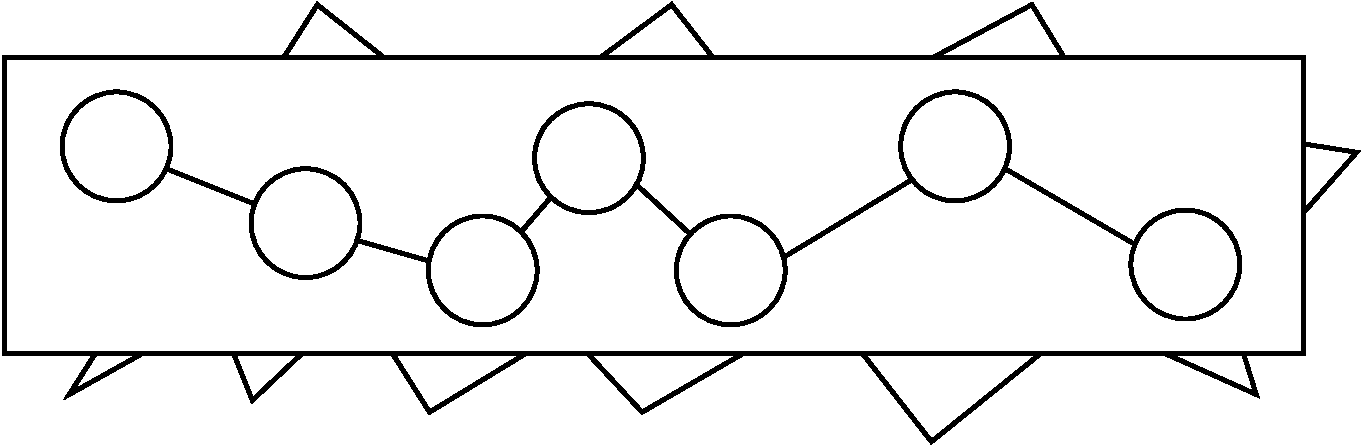
\includegraphics[width=0.9\textwidth]{test.pdf}
}
\caption{A nice caption. The larger width allows for more text without
taking too much space.}
\label{Fig2}
\end{figure*}


\section{Basic Rules for Using Latex}

First, we want to refer to the figures and the introduction.
See Figure~\ref{TUM} for the first floating figure with column width,
and Figure~\ref{Fig2} for the one using the full page width.
And here, we want to put a reference to the introduction which is
Section~\ref{introduction}.

In translating this template from German to English, I decided to
stop here. There is not really much to get from the German text
following. Anything Latex-related can also be looked up on the
net. There is a {\it huge} number of tutorials, and so on.

Please do not use to much different font sizes and styles. It should
be completely enough to go to {\em italic mode} for emphasizing something,
such as newly introduced terms.
You can refer to other parts of your paper (e.g. see 
Sec.~\ref{introduction}).
Quoting in Latex is done ``this way''.
Further, you may have problems with punctation characters.
Most of them just need to be prefixed by a backslash, for others you may
temporarily switch to math mode:
\$ \& \% \# \{ \} [ ] \_ @ \S $<$ $>$ $\backslash$ @ \textasciitilde /
    
Talking about math mode: you can do some very nice things this way:

\begin{equation}
a^2 + b^2 = c^2
\label{Pythagoras}
\end{equation}

Again, refering to this equation is easy (see Eq.~\ref{Pythagoras}).
If you do not need numbering for equations, use the {\em displaymath}
environment:

\begin{displaymath}
x_{1,2} = \frac{-b \pm \sqrt{b^2-4ac}}{2a}\\
\end{displaymath}

Short equations simply can be used within the regular text flow, such
as with $x \to \infty$. Obviously, math is fun with Latex.


\section{Enumerations}

Enumerations using bullet points:

\begin{itemize}
	\item this is the first item of this list of interesting facts,
	\item second item,
	\item and the last one.
\end{itemize}

They also can be numbered:

\begin{enumerate}
	\item item one,
	\item item two,
	\item item three.
\end{enumerate}

As shown, numbers always should be written out in the text, unless the
belong to a title or a formula.

\section{Literature}

At the end of your paper, you should have a nice list of used
literature. For scientific papers, this actually is needed. You always
use other works as base for your own. Usually, you are not the only
one thinking about a given difficult problem, so there is always
related work which {\em must} be cited if known to the author.

Further, if you want to copy relevant sentences from an
original paper, you {\em have} to cite them correctly, for example
in this way:

\begin{quote}
	``I think there is a world market for maybe five computers.''
	(T.J. Watson, IBM, 1943)
\end{quote}

The rest of the work (especially all the regular text) must be
written/phrased by you. If you write about some results or fact
stated in another paper, you should refer to it.
The `Analytical Engine'' --- a mechanical calculation machine ---
created by Charles Babbage in the year 1838 was based on the decimal
system
% use \cite to refer to papers from seminarpaper.bib
% this file is processed by bibtex, and it automatically adds numbering
\cite{Brom98}.

\section{Figures and Tables}

No need to understand the following text.

Figures can span either one column (see Figure~\ref{TUM}) or the full
page width (see Figure~\ref{Fig2}).
Latex automatically tries to find the best place for these floating
figures. To influence that, you may move the figure a bit to the front
of your text.
As can be seen in Figure~\ref{TUM}, using images usually results in very
bad quality. Better use vector formats: draw the figures with
{\em xfig} or {\em inkscape}, and save them as PDF. As example of
this procedure, see Figure~\ref{Fig2}).

% Narrow tables (just one column) have no * at the end
\begin{table*}

\begin{center}
% arguments:
% c = center
% l = left
% r = right (z. B. for cash)
% p = columns with fixed width, using block layout
% | = vertical line
\begin{tabular}{|l|p{2cm}|c|c|c|c|c|r|}
% horizontal line
\hline
% & means: next column
% \\ means: next row
	& Column 1 & Column 2 & Column 3 & Column 4& Column 5& Column 6& 
Amount\\
\hline
Row 1 & This column has a maximal width of 2 cm.& X & X& X& X& X& 126,00\\
\hline
Row 2 & & \multicolumn{3}{p{5cm}|}{This entry occupies three columns.}& X &X 
& 8,00\\
\hline
\multicolumn{7}{|l}{Sum} &134,00\\
\hline
\end{tabular}
\end{center}

\caption{This is the caption of the table.}
% label is for this table
\label{Tab1}

\end{table*}

Similar to figures, tables can be referred to in the text (see 
Tab.~\ref{Tab1}). However, sometimes it is useful to embed tables directly in 
the regular text flow:

\begin{center}
\begin{tabular}{|c|c|c|}
\hline
	& Column 1 & Column 2 \\
\hline
Row 1 & & \\
Row 1 & & \\
\hline
\end{tabular}
\end{center}


\section{Summary}
\label{summary}

The summary shortly repeats the core ideas and results from the
previous text. If the reader has problems understanding the summary
he knows that he should go back to the relevant sections.
Thus, the last section should consist of:

\begin{itemize}
	\item a summary,
	\item an evaluation of what was done, importance of this work,
	\item what is left, what still needs to be done,
	\item short outlook into the future.
\end{itemize}

Last but not least, we can explain anything missing yet in the evaluation
done in this paper. This allows to refer to what readers can expect from
authors in the future.

% Put citations from bibtex into References section which were not
% explicity cited.
\nocite{robotron,
stonx,vice,650sim,herculessim,zib,4004,thermal1,thermal2,rojas}


\bibliographystyle{plain}
% Literature sources are to be found in seminarpaper.bib
\bibliography{iot_report}
\end{document}
